\documentclass[border=1mm]{standalone}
% \usepackage[margin=2.5cm]{geometry}

\usepackage{graphicx,tikz,tikz-layers} 
\usetikzlibrary{decorations.markings,calc,positioning,arrows,shapes.geometric,arrows.meta}

\colorlet{myred}{red!80!black}
\colorlet{myblue}{blue!80!black}
\colorlet{mybluee}{myblue!80!black}
\colorlet{mygreen}{green!60!black}
\colorlet{myorange}{orange!70!red!60!black}
\colorlet{mydarkred}{red!20!black}
\colorlet{mydarkblue}{blue!40!black}
\colorlet{mydarkgreen}{green!20!black}




\begin{document}

% \resizebox{\textwidth}{!}{
\tikz[font=\small,scale=1, every node/.style={outer sep=0pt, inner sep=0pt}, w/.style={minimum width=#1},h/.style={minimum height=#1},s/.style={minimum size=#1}, eu/.style={shorten >=#1},ed/.style={shorten <=#1},line join=round]
{
\tikzset{>={Latex[length=1.5mm, width=1.25mm]}}

\node[draw, w=1.75cm, h=.35cm] (a) {$4\times 4$};
\node[draw, w=1.75cm, h=.35cm, below=6.4cm of a] (b) {$4\times 4$};

\node[draw, w=1.75cm, h=.35cm, right=1.5cm of a] (c) {$4\times 4$};
\node[draw, w=1.75cm, h=.35cm] (d) at (c|-b) {$4\times 4$};
\node[draw, w=2cm, h=.35cm, below=1mm of c] (88a) {$8\times 8$};
\node[draw, w=2cm, h=.35cm, above=1mm of d] (88b) {$8\times 8$};

\node[draw, w=1.75cm, h=.35cm, right=6cm of c] (e) {$4\times 4$};
\node[draw, w=1.75cm, h=.35cm] (f) at (e|-b) {$4\times 4$};
\node[draw, w=2cm, h=.2cm, below=1mm of e] (a1) {};
\node[draw, w=2.35cm, h=.2cm, below=1mm of a1] (a2) {};
\node[draw, w=2.7cm, h=.2cm, below=1mm of a2] (a3) {};
\node[draw, w=3.05cm, h=.2cm, below=1mm of a3] (a4) {};
\node[draw, w=3.4cm, h=.2cm, below=1mm of a4] (a5) {};
\node[draw, w=3.75cm, h=.2cm, below=1mm of a5] (a6) {};
\node[draw, w=4.1cm, h=.2cm, below=1mm of a6] (a7) {};
\node[draw, w=4.45cm, h=.35cm, below=1mm of a7] (a8) {$1024\times 1024$};


\node[draw, w=2cm, h=.2cm, above=1mm of f] (b1) {};
\node[draw, w=2.35cm, h=.2cm, above=1mm of b1] (b2) {};
\node[draw, w=2.7cm, h=.2cm, above=1mm of b2] (b3) {};
\node[draw, w=3.05cm, h=.2cm, above=1mm of b3] (b4) {};
\node[draw, w=3.4cm, h=.2cm, above=1mm of b4] (b5) {};
\node[draw, w=3.75cm, h=.2cm, above=1mm of b5] (b6) {};
\node[draw, w=4.1cm, h=.2cm, above=1mm of b6] (b7) {};
\node[draw, w=4.45cm, h=.35cm, above=1mm of b7] (b8) {$1024\times 1024$};



% Arrows and labels
\draw[dashed, gray] ([xshift=-1cm]$(a)!.5!(b)$)--coordinate[pos=1] (v) ([xshift=2cm]$(c)!.5!(d)$);
\draw[dashed, gray] ([xshift=-3cm]$(e)!.5!(f)$)--coordinate[pos=0] (u) ([xshift=2cm]$(e)!.5!(f)$);

\node[scale=1.75] at ($(u)!.5!(v)$) {$\ldots$};

\node[above=4mm of a] (lat1) {Latent};
\node[above=4mm of c] (lat2) {Latent};
\node[above=4mm of e] (lat3) {Latent};
\draw[->, ed=.7mm] (lat1)--(a);
\draw[->, ed=.7mm] (lat2)--(c);
\draw[->, ed=.7mm] (lat3)--(e);

\draw[->] ($(b.south west)+(-.5,-.25)$)--node[fill=white, inner xsep=3mm, pos=.6] {Training progresses} ($(f.south east)+(1,-.25)$);

\draw[->, dotted] (a)--(b);
\draw[->, dotted] (88a)--(88b);
\draw[->, dotted] (a8)--(b8);
\draw[->, dotted] ($(u-|b.north)+(.3,-.3)$)--node[pos=0, right=1mm] {\scriptsize Reals} ($(b.north)+(.3,0)$);
\draw[->, dotted] ($(u-|d.north)+(.3,-.3)$)--node[pos=0, right=1mm] {\scriptsize Reals} ($(88b.north)+(.3,0)$);  
\draw[->, dotted] ($(u-|f.north)+(.3,-.1)$)--node[pos=0.3, right=2mm] {\scriptsize Reals} ($(b8.north)+(.3,0)$);

\node[above left=.5cm of a] {\large\textbf{G}};
\node[above left=.5cm of b] {\large\textbf{D}};

\node[anchor=east] at ([xshift=-.5mm]u-|a.south) {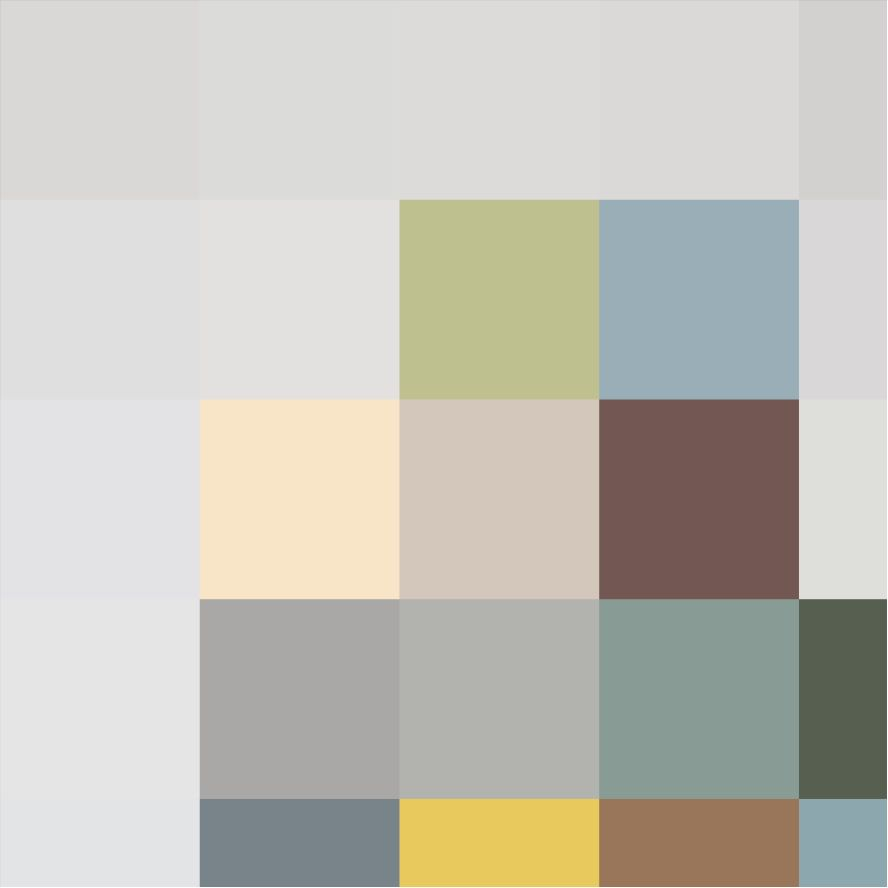
\includegraphics[width=1cm]{images/parrot1.jpeg}};
\node[anchor=east] at ([xshift=-.5mm]u-|c.south) {
\includegraphics[width=1cm]{images/parrot2.jpeg}};
\node[anchor=east] at ([xshift=-.5mm]u-|e.south) {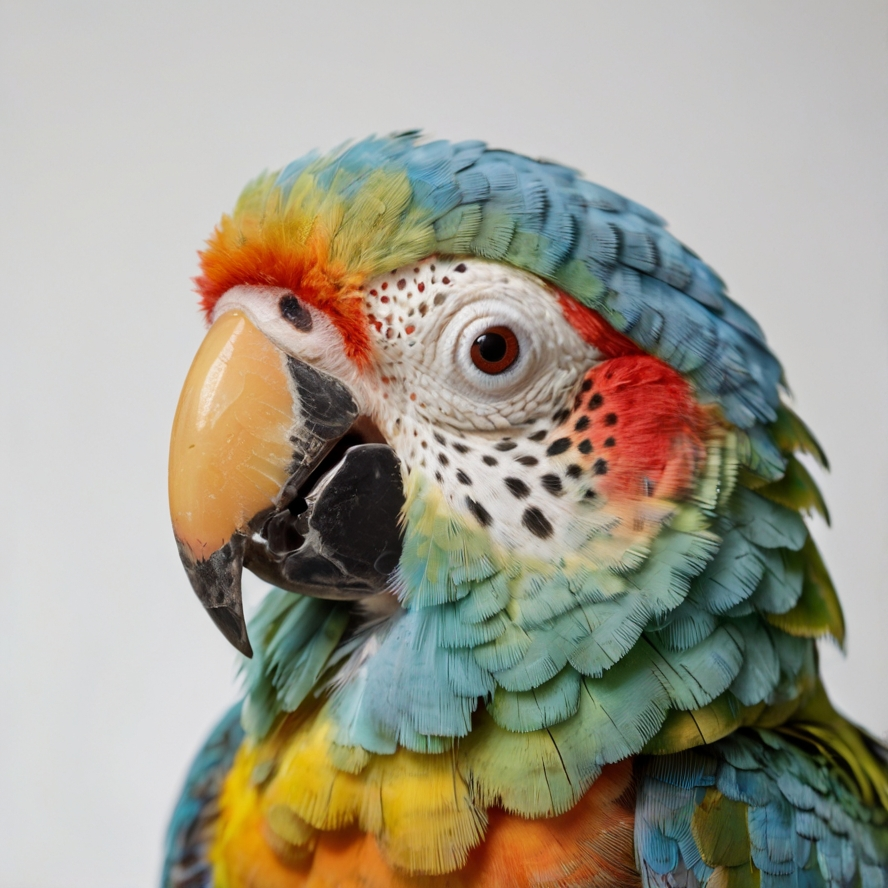
\includegraphics[width=1cm]{images/parrot3.jpg}};
}
% }
\end{document}
